\documentclass[a4paper]{article}

\usepackage{a4wide}
\usepackage{listings}
\usepackage{inconsolata}
\usepackage{url}

%\VignetteIndexEntry{Using RUnBBayes}

%----------------------------------------------------------------------------------------
%  DOCUMENT INFORMATION
%----------------------------------------------------------------------------------------

\title{Bayesian networks in R with RUnBBayes package} % Title

%\author{John \textsc{Smith}} % Author name

\date{\today} % Date for the report

\usepackage{Sweave}
\begin{document}
\Sconcordance{concordance:tutorial.tex:tutorial.Rnw:%
1 19 1 1 0 58 1 1 2 1 0 1 3 1 0 1 2 1 0 1 2 1 0 1 2 1 0 1 2 1 0 1 2 1 0 %
1 2 1 0 1 2 4 0 1 2 2 1 1 3 2 0 1 1 9 0 1 2 5 1 1 2 1 0 2 1 14 0 1 2 4 %
1 1 2 1 0 1 1 14 0 1 2 4 1 1 2 1 0 1 1 35 0 1 2 11 0 1 2 6 0 1 2 3 1 1 %
2 1 0 1 1 12 0 1 2 2 1 1 3 2 0 1 1 8 0 1 2 2 1 1 2 1 0 3 1 7 0 1 2 2 1 %
8 0 1 2 5 1 1 3 2 0 1 1 3 0 1 2 14 1}


\maketitle % Insert the title, author and date

\begin{center}
\begin{tabular}{l r}
Developers: & Fernando Santos \\ % Partner names
& Yuri Lavinas \\
& Samuel Pala \\
& Diego Marques \\
& Pedro Henrique \\
Instructor: & Rommel Carvalho % Instructor/supervisor
\end{tabular}
\end{center}

% If you wish to include an abstract, uncomment the lines below
% \begin{abstract}
% Abstract text
% \end{abstract}

%----------------------------------------------------------------------------------------
%  SECTION 1
%----------------------------------------------------------------------------------------

\section{Introduction}

The RUnBBayes package provides access to some functionalities of the UnBBayes framework. UnBBayes (\url{http://unbbayes.sourceforge.net/}) is an open source software for modeling, learning and reasoning upon probabilistic networks developed in Java. Making use of rJava, this package provides an interface to implement probabilistic networks within R.

% If you have more than one objective, uncomment the below:
%\begin{description}
%\item[First Objective] \hfill \\
%Objective 1 text
%\item[Second Objective] \hfill \\
%Objective 2 text
%\end{description}



\section{The chest clinic example}

This section explains how to use RUnBBayes in the chest clinic example of Lauritzen and Spiegelhalter (1988) (Figure~\ref{fig:asia}). As stated by Lauritzen and Spiegelhalter (1988):

\begin{quotation}
Shortness-of-breath (dyspnoea) may be due to tuberculosis, lung cancer or bronchitis, or none of them, or more than one of them. A recent visit to Asia increases the chances of tuberculosis, while smoking is known to be a risk factor for both lung cancer and bronchitis. The results of a single chest X-ray do not discriminate between lung cancer and tuberculosis, as neither does the presence or absence of dyspnoea.
\end{quotation}

\begin{figure}[ht!]
\centering
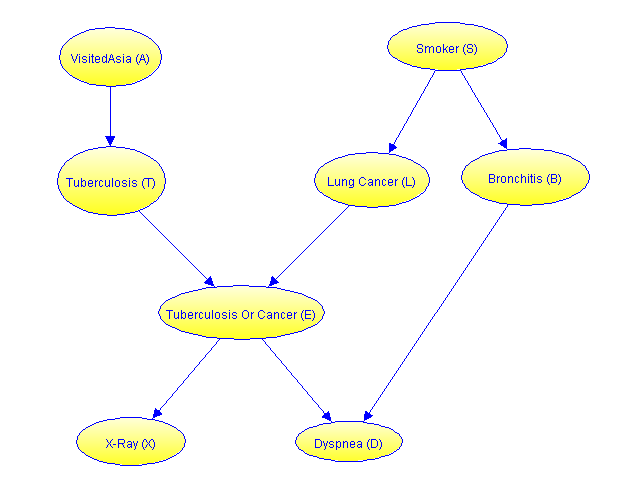
\includegraphics[width=90mm]{chest-clinic.png}
\caption{Chest clinic example}
\label{fig:asia}
\end{figure}


\subsection{Defining the network nodes}

We can create a network by defining its nodes, together with their conditional probabilities and their state. 

\begin{Schunk}
\begin{Sinput}
> library(runbbayes)
> node.a = createNodeInfo(~asia, prob=c(0.01, 0.99), 
+                         states=c("yes","no"))
> node.t = createNodeInfo(~tub|asia, prob=c(0.05, 0.95, 0.01, 0.99),
+                         states=c("yes","no"))
> node.s = createNodeInfo(~smoke, prob=c(0.5,0.5), 
+                         states=c("yes","no"))
> node.l = createNodeInfo(~lung|smoke, prob=c(0.1, 0.9, 0.01, 0.99), 
+                         states=c("yes","no"))
> node.b = createNodeInfo(~bronc|smoke, prob=c(0.6, 0.4, 0.3, 0.7), 
+                         states=c("yes","no"))
> node.e = createNodeInfo(~either|lung:tub,prob=c(1,0,1,0,1,0,0,1),
+                         states=c("yes","no"))
> node.x = createNodeInfo(~xray|either, prob=c(0.98, 0.02, 0.05, 0.95), 
+                         states=c("yes","no"))
> node.d = createNodeInfo(~dysp|bronc:either, prob=c(0.9, 0.1, 0.7, 0.3, 0.8, 0.2, 0.1, 0.9), 
+                         states=c("yes", "no"))
\end{Sinput}
\end{Schunk}

Each of these calls will return a "nodeinfo" structure.

\begin{Schunk}
\begin{Sinput}
> node.a = createNodeInfo(~asia, prob=c(0.01, 0.99), 
+                         states=c("yes","no"))
> node.a
\end{Sinput}
\begin{Soutput}
Node:           asia
Parents:        NA
Probabilities:  0.01, 0.99
States:         yes, no
\end{Soutput}
\end{Schunk}

\subsection{Compiling the network}

Create a probabilistic network, from a node list.
Compile list of conditional probability tables and create the network.

\begin{Schunk}
\begin{Sinput}
> nodeList = list(node.a, node.t, node.s, node.l, node.b, node.e, node.x, node.d)
> network = createNetwork(nodeList, compile=TRUE)
> network
\end{Sinput}
\begin{Soutput}
Compiled: TRUE
P ( asia )
P ( tub | asia )
P ( smoke )
P ( lung | smoke )
P ( bronc | smoke )
P ( either | lung tub )
P ( xray | either )
P ( dysp | bronc either )
\end{Soutput}
\end{Schunk}

Setting compile as true, gives you a compiled network. Otherwise, the network won't
be compiled by default.So, it's necessary to use the compileNetwork function as an
option to build the junction tree.

\begin{Schunk}
\begin{Sinput}
> netCompiled = compileNetwork(network)
> netCompiled
\end{Sinput}
\begin{Soutput}
Compiled: TRUE
P ( asia )
P ( tub | asia )
P ( smoke )
P ( lung | smoke )
P ( bronc | smoke )
P ( either | lung tub )
P ( xray | either )
P ( dysp | bronc either )
\end{Soutput}
\end{Schunk}

\subsection{Querying the network}

1. The network can be queried to return the priori probabilities of all nodes:

\begin{Schunk}
\begin{Sinput}
> prioriProb = queryNetwork(network)
> prioriProb
\end{Sinput}
\begin{Soutput}
$asia
		yes		no
		0.01		0.99

$tub
		yes		no
		0.0104		0.9896

$smoke
		yes		no
		0.5		0.5

$lung
		yes		no
		0.055		0.945

$bronc
		yes		no
		0.45		0.55

$either
		yes		no
		0.0648		0.9352

$xray
		yes		no
		0.1103		0.8897

$dysp
		yes		no
		0.436		0.564
\end{Soutput}
\begin{Sinput}
> prioriProb$xray
\end{Sinput}
\begin{Soutput}
$yes

		0.1103

$no

		0.8897
\end{Soutput}
\begin{Sinput}
> prioriProb$xray$yes
\end{Sinput}
\begin{Soutput}
[1] 0.1103
\end{Soutput}
\end{Schunk}


2. The network can be queried to return the priori probabilities of some specific nodes:

\begin{Schunk}
\begin{Sinput}
> prioriProb = queryNetwork(network, c("bronc", "dysp"))
> prioriProb
\end{Sinput}
\begin{Soutput}
$bronc
		yes		no
		0.45		0.55

$dysp
		yes		no
		0.436		0.564
\end{Soutput}
\end{Schunk}

3. The network can return the posteriori probabilities of some event given some evidences without modifying the current network object:

\begin{Schunk}
\begin{Sinput}
> posterioriProb = queryNetwork(network, c("either"), list(c("asia",
+ "yes"), c("smoke","no")))
> posterioriProb
\end{Sinput}
\begin{Soutput}
$either
		yes		no
		0.0595		0.9405
\end{Soutput}
\end{Schunk}

4. Evidences can be set and reset in the network:

\begin{Schunk}
\begin{Sinput}
> network = setEvidence(network, list(c("asia", "yes"), c("smoke", "no")))
> network = propagateEvidence(network)
> posterioriProb = queryNetwork(network, c("dysp", "yes"))
> posterioriProb
\end{Sinput}
\begin{Soutput}
$dysp
		yes		no
		0.3368		0.6632
\end{Soutput}
\begin{Sinput}
> network = resetEvidence(network)
> prioriProb = queryNetwork(network, c("dysp", "yes"))
> prioriProb
\end{Sinput}
\begin{Soutput}
$dysp
		yes		no
		0.436		0.564
\end{Soutput}
\end{Schunk}


\subsection{Updating the network}

1. Nodes can be added or removed from a compiled network:

\begin{Schunk}
\begin{Sinput}
> network = addNode(network, ~asthma|smoke, prob = c(0.6, 0.4, 0.85, 0.15), states = c("yes",
+ "no"))
> network = removeNode(network, "asthma")
\end{Sinput}
\end{Schunk}



%----------------------------------------------------------------------------------------
%	BIBLIOGRAPHY
%----------------------------------------------------------------------------------------

\bibliographystyle{unsrt}

\bibliography{sample}

%----------------------------------------------------------------------------------------


\end{document}
